\section{Phân tích yêu cầu đối với hệ thống RAG}

RAG (Retrieval-Augmented Generation) là kỹ thuật kết hợp giữa truy xuất thông tin và sinh câu trả lời bằng mô hình ngôn ngữ.

\subsection{Vai trò của RAG trong hệ thống}
\begin{table}[H]
\centering
\caption{Vai trò của RAG}
\label{tab:rag_roles}
\begin{tabular}{|p{4cm}|p{8cm}|}
\hline
\textbf{Vai trò} & \textbf{Mô tả} \\ \hline
Truy xuất tài liệu & Tìm đoạn nội dung liên quan đến câu hỏi \\ \hline
Bổ sung tri thức & Hỗ trợ các câu hỏi không nằm trong intent cố định \\ \hline
Giảm trả lời sai & Câu trả lời dựa trên bằng chứng tìm được \\ \hline
Hỗ trợ trích dẫn & Cho phép hiển thị nguồn tham khảo \\ \hline
Dễ cập nhật & Chỉ cần upload tài liệu mới và index lại \\ \hline
\end{tabular}
\end{table}

\subsection{Yêu cầu đối với dữ liệu đầu vào}
\begin{table}[H]
\centering
\caption{Yêu cầu đối với dữ liệu RAG đầu vào}
\label{tab:rag_input_requirements}
\begin{tabular}{|p{4cm}|p{8cm}|}
\hline
\textbf{Yêu cầu} & \textbf{Mô tả} \\ \hline
Nguồn chính thống & Tài liệu lấy từ trường hoặc đơn vị tuyển sinh \\ \hline
Định dạng hỗ trợ & PDF, DOCX, TXT, HTML hoặc văn bản thuần \\ \hline
Nội dung rõ ràng & Có tiêu đề, mục lục, bảng biểu nếu cần \\ \hline
Có thông tin năm & Tài liệu nên gắn với năm tuyển sinh \\ \hline
Được kiểm duyệt & Quản trị viên cần xác nhận trước khi sử dụng \\ \hline
\end{tabular}
\end{table}

\subsection{Yêu cầu đối với quá trình indexing}
\begin{enumerate}
    \item Upload tài liệu.
    \item Trích xuất văn bản từ tài liệu.
    \item Làm sạch nội dung.
    \item Chia văn bản thành các đoạn nhỏ.
    \item Gắn metadata cho từng đoạn.
    \item Sinh embedding.
    \item Lưu vào vector store.
    \item Lưu thông tin tài liệu vào document store.
\end{enumerate}

\begin{figure}[H]
    \centering
    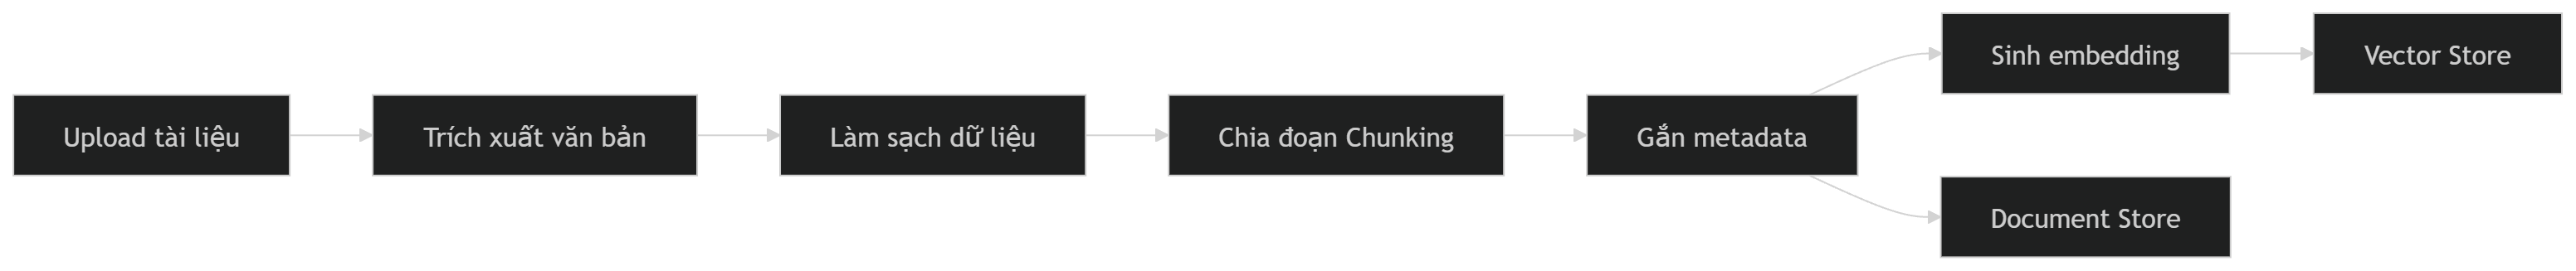
\includegraphics[width=\textwidth]{content/source/Hình 2.5 Luồng Indexing Flow của hệ thống RAG..png}
    \caption{Luồng indexing của hệ thống RAG}
    \label{fig:rag_indexing_flow}
\end{figure}

\subsection{Yêu cầu đối với quá trình truy vấn}
\begin{enumerate}
    \item Nhận câu hỏi từ chatbot.
    \item Chuẩn hóa câu hỏi.
    \item Sinh embedding cho câu hỏi.
    \item Truy xuất các đoạn liên quan từ vector store.
    \item Có thể tái xếp hạng kết quả nếu cần.
    \item Tạo prompt gồm câu hỏi và bằng chứng.
    \item Gọi mô hình sinh câu trả lời.
    \item Trả lời người dùng kèm nguồn tham khảo.
\end{enumerate}

\begin{figure}[H]
    \centering
    
\includegraphics[width=\textwidth]{content/source/Hình 2.6 Luồng Query Flow của hệ thống RAG.png}
    \caption{Luồng truy vấn của hệ thống RAG}
    \label{fig:rag_query_flow}
\end{figure}

\subsection{Yêu cầu về metadata}
\begin{table}[H]
\centering
\caption{Metadata đề xuất cho mỗi đoạn tài liệu}
\label{tab:rag_metadata}
\begin{tabular}{|p{3.6cm}|p{8.4cm}|}
\hline
\textbf{Metadata} & \textbf{Ý nghĩa} \\ \hline
document\_id & Mã tài liệu \\ \hline
document\_name & Tên tài liệu \\ \hline
year & Năm tuyển sinh \\ \hline
source\_type & Loại tài liệu: đề án, thông báo, quy chế \\ \hline
page\_number & Số trang \\ \hline
section\_title & Tiêu đề mục \\ \hline
created\_at & Thời điểm thêm vào hệ thống \\ \hline
status & Trạng thái: đang dùng, nháp, đã khóa \\ \hline
\end{tabular}
\end{table}

\subsection{Yêu cầu về chất lượng RAG}
\begin{table}[H]
\centering
\caption{Yêu cầu chất lượng cho hệ thống RAG}
\label{tab:rag_quality}
\begin{tabular}{|p{2.2cm}|p{9.8cm}|}
\hline
\textbf{Mã} & \textbf{Nội dung} \\ \hline
RAG-01 & Truy xuất đúng đoạn liên quan đến câu hỏi \\ \hline
RAG-02 & Ưu tiên tài liệu mới nhất hoặc đúng năm người dùng hỏi \\ \hline
RAG-03 & Câu trả lời phải dựa trên bằng chứng truy xuất \\ \hline
RAG-04 & Không sinh câu trả lời nếu không tìm thấy bằng chứng phù hợp \\ \hline
RAG-05 & Có thể hiển thị nguồn tài liệu để người dùng kiểm tra \\ \hline
RAG-06 & Hỗ trợ cập nhật hoặc xóa tài liệu lỗi thời \\ \hline
RAG-07 & Cho phép quản trị viên index lại tài liệu khi có thay đổi \\ \hline
\end{tabular}
\end{table}
